\documentclass[aspectratio=1610]{beamer}

\usepackage[utf8]{inputenc}
\usepackage[T1]{fontenc}
\usepackage{amsmath,amssymb}
\usepackage{hyperref}
\usepackage{tikz}
\usetikzlibrary{calc, positioning, arrows.meta, shapes.geometric}
\usepackage{multirow}
\usepackage{fontawesome}
\usepackage[normalem]{ulem}

% Liens bleus soulignés
\hypersetup{colorlinks=false, urlbordercolor=blue, pdfborderstyle={/S/U/W 1}}
\let\hrefnoformat\href
\renewcommand{\href}[2]{\hrefnoformat{#1}{\textcolor{blue}{\underline{#2}}}}

% Bandeau cliquable en haut de chaque slide
\addtobeamertemplate{headline}{}{%
  \begin{tikzpicture}[remember picture,overlay]
    \node[anchor=north,inner sep=0pt,yshift=0.5pt] at (current page.north) {%
      \hrefnoformat{https://zknox.com}{\includegraphics[width=\paperwidth,height=0.8cm,keepaspectratio=false]{bandeau.png}}%
    };
  \end{tikzpicture}%
}

% Décaler le contenu et supprimer la ligne de séparation
\setbeamercolor{frametitle}{fg=black,bg=white}
\setbeamertemplate{frametitle}{\vspace{0.8cm}\insertframetitle}

\setbeamertemplate{navigation symbols}{%
    \usebeamerfont{footline}%
    \usebeamercolor[fg]{footline}%
    \hspace{1em}%
    \insertframenumber/\inserttotalframenumber
}
\setbeamercolor{footline}{fg=black}

\date{February 4, 2026}
\title{Post-Quantum Transaction Signatures}
\subtitle{PQTS Breakout Room --- ZKNOX contributions}
\author{Renaud Dubois, Simon Masson, Nicolas Bacca\\[0.5em]
\includegraphics[height=3em]{zknox.png}\\[0.3em]
{\footnotesize Slides: \href{https://github.com/ZKNoxHQ/Communications/tree/main/pqts-breakout}{github.com/ZKNoxHQ/Communications/pqts-breakout}}}

\begin{document}

%% ============================================================
%% SLIDE 1: TITRE
%% ============================================================
\begin{frame}
  \vspace{0.8cm}
  \maketitle
\end{frame}

%% ============================================================
%% SLIDE 2: WHAT WE HAVE
%% ============================================================
\begin{frame}{What We Have Today --- Full Operational Suite with Dapp Integration}

\begin{columns}[T]
\begin{column}{0.55\textwidth}
\textbf{Precompile EIPs (deployed on testnet):}
\begin{itemize}
  \item \href{https://eips.ethereum.org/EIPS/eip-8051}{EIP-8051}: ML-DSA (Dilithium) precompile
  \item \href{https://eips.ethereum.org/EIPS/eip-8052}{EIP-8052}: FN-DSA (Falcon) precompile
  \item Ethereum-optimized variants (Keccak PRNG)
\end{itemize}

\vspace{0.6em}
\textbf{Signer implementations:}
\begin{itemize}
  \item ML-DSA on Ledger hardware wallet
  \item Falcon software signer
  \item \href{https://github.com/ZKNoxHQ/PQBIP39}{PQ-BIP39} key derivation\\
        {\small (\href{https://ethresear.ch/t/how-to-hard-fork-to-save-most-users-funds-in-a-quantum-emergency/18901}{zkProof of seed})}
\end{itemize}
\end{column}

\begin{column}{0.42\textwidth}
\textbf{Hybrid \& agile verifier (ERC-4337):}
\begin{itemize}
  \item ECDSA (k1/r1) + ML-DSA/FN-DSA
  \item ETH-optimized or NIST-native
  \item Modular, swappable verifiers
\end{itemize}

\vspace{0.6em}
\textbf{Full stack:}\\[0.3em]
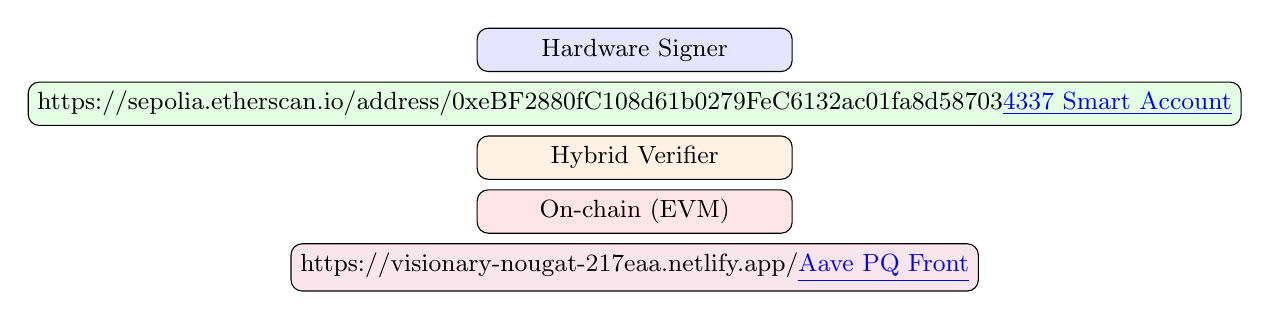
\begin{tikzpicture}[
  every node/.style={draw, rounded corners, minimum width=4cm, minimum height=0.55cm, font=\small},
  node distance=0.12cm
]
\node (hw) [fill=blue!10] {Hardware Signer};
\node (sa) [below=of hw, fill=green!10] {\href{https://sepolia.etherscan.io/address/0xeBF2880fC108d61b0279FeC6132ac01fa8d58703}{4337 Smart Account}};
\node (vc) [below=of sa, fill=orange!10] {Hybrid Verifier};
\node (ch) [below=of vc, fill=red!10] {On-chain (EVM)};
\node (fr) [below=of ch, fill=purple!10] {\href{https://visionary-nougat-217eaa.netlify.app/}{Aave PQ Front}};
\end{tikzpicture}
\end{column}
\end{columns}

\end{frame}

%% ============================================================
%% SLIDE 3: PROTECT HIGH VALUE USE CASES TODAY
%% ============================================================
\begin{frame}{Protecting High-Value Use Cases \textbf{Today}}

\textbf{Key insight:} We don't need precompiles to start protecting assets \emph{now}.\\
Pure Solidity verification works --- and at current gas prices, it's affordable.

\vspace{0.3em}

\begin{center}
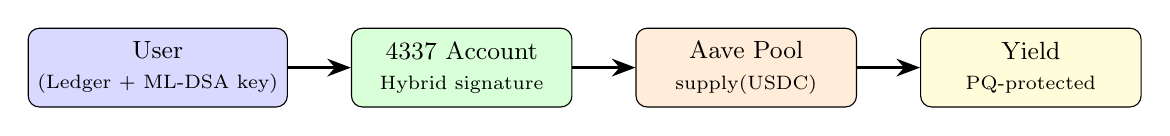
\begin{tikzpicture}[
  box/.style={draw, rounded corners, minimum width=2.8cm, minimum height=1cm, align=center, font=\small},
  arr/.style={-{Stealth[length=3mm]}, thick},
  node distance=0.8cm
]
\node (user) [box, fill=blue!15] {User\\{\scriptsize (Ledger + ML-DSA key)}};
\node (sa)   [box, right=of user, fill=green!15] {4337 Account\\{\scriptsize Hybrid signature}};
\node (aave) [box, right=of sa, fill=orange!15] {Aave Pool\\{\scriptsize supply(USDC)}};
\node (yield)[box, right=of aave, fill=yellow!15] {Yield\\{\scriptsize PQ-protected}};

\draw[arr] (user) -- (sa);
\draw[arr] (sa) -- (aave);
\draw[arr] (aave) -- (yield);
\end{tikzpicture}
\end{center}

\vspace{0.3em}

\begin{center}
\renewcommand{\arraystretch}{1.3}
{\small
\begin{tabular}{l c c}
\hline
\textbf{Scheme} & \textbf{Gas (Solidity)} & \textbf{Cost @0.55 gwei, ETH=\$2322} \\
\hline
ML-DSA (NIST)     & 13.0M gas & \$16.60 \\
ML-DSA-ETH        & 8.3M gas  & \$10.60 \\
Falcon (NIST)     & 4.1M gas  & \$5.24 \\
Falcon-ETH        & 1.6M gas  & \textbf{\$2.04} \\
\hline
\end{tabular}
}
\end{center}

\vspace{0.3em}

\textbf{Use cases (no precompile needed):}
governance contracts, treasury management, DeFi yield positions (Aave, Compound), multisig upgrades --- high value, low frequency.

\end{frame}

%% ============================================================
%% SLIDE 4: WHY WE NEED PRECOMPILES
%% ============================================================
\begin{frame}{Why We Need Precompiles}

With precompiles, PQ signature verification cost becomes comparable to ECDSA.\\
The dominant cost of a PQ transaction is then the \textbf{UserOp handling itself}, not the cryptography.

\end{frame}

%% ============================================================
%% SLIDES SIMON
%% ============================================================

\begin{frame}{NIST candidates (pros and cons)}
  Standardization since 2016... and \xout{the winner is} the winners are:
  \begin{itemize}
    \item \textbf{Dilithium -- ML-DSA}, based on lattices,
    \item \textbf{Falcon -- FN-DSA}, based on lattices,
    \item SPHINCS -- SLH-DSA, based on hash functions (big and expensive)
  \end{itemize}

  How to choose?\pause
  \begin{center}
    \begin{tabular}{|l|c|c|}
      \hline
      & \textbf{ML-DSA} & \textbf{FN-DSA}\\
      \hline
      \textbf{EIP} &  \href{
        https://github.com/ethereum/EIPs/blob/master/EIPS/eip-8051.md
      }{8051} &
        \href{
        https://github.com/ethereum/EIPs/blob/master/EIPS/eip-8052.md
      }{8052} \\
      \hline
      \textbf{Public key} & \textcolor{orange}{1312B} & \textcolor{green}{897B} \\
      \textbf{Signature}  & \textcolor{orange}{2420B} & \textcolor{green}{666B} \\
      \hline
      \textbf{On-chain cost} &\textcolor{orange}{13.0M gas} {\tiny (8.3M gas)} &\textcolor{orange}{4.1M gas} {\tiny (1.6M gas)}\\
      \textbf{(with Precompile)} &\textcolor{orange}{4500 gas}  &\textcolor{orange}{3000 gas}\\
      
      \hline
      \textbf{Standardized?}  &        \textcolor{green}{FIPS 204} &   \textcolor{red}{not yet} (since 2 years) \\
      \textbf{Signer implementation} & \textcolor{green}{Easy, many} & Tricky, floating point\\
      \textbf{Hardware integration} &  \textcolor{green}{Done} &       High RAM requirements\\
      \textbf{Industrial integration} & Passkey, Apple (soon) & Luna HSM (no memory constraint)\\
      \hline
      \textbf{ZK variant} & Possible & \textcolor{red}{Overstretch attacks}\\
      \hline
    \end{tabular}
  \end{center}
\end{frame}

\begin{frame}{EIPs 8051 and 8052}
  \begin{itemize}
    \item \textbf{EIP 8051}: \href{
        https://github.com/ethereum/EIPs/blob/master/EIPS/eip-8051.md
      }{link}
    \begin{itemize}
      \item Two precompiles:
      \begin{itemize}
        \item MLDSA: NIST-compliant with SHAKE256\\
        (verification: 13.0 M gas, not far from the tx limit of 16M!).
        \item MLDSA-ETH: replacement with a counter-mode Keccak PRNG\\
        (verification: 8.3M gas).
      \end{itemize}
      \item Test vector provided (generated from NIST reference implementation).
      \item Integrated into a 4337 hybrid (MLDSA + ECDSA) account.\\
      
    \end{itemize}
    \pause
    \item \textbf{EIP 8052}: \href{
        https://github.com/ethereum/EIPs/blob/master/EIPS/eip-8052.md
      }{link}
    \begin{itemize}
      \item Separation of the hash part and the polynomial arithmetic:
      \begin{itemize}
        \item FALCON: NIST-compliant with SHAKE256\\
        (verification: 4.1M gas).
        \item ETH-FALCON: replacement with a counter-mode Keccak PRNG\\
        (verification: 1.6M gas).
      \end{itemize}
      \item Precompiles for FALCON-CORE and HASH-TO-POINT (one for Shake256, one for KeccakPRNG).
      \item Test vector provided (generated from NIST reference implementation).
      \item Integration in a 4337 account in progress...
    \end{itemize}
  \end{itemize}
\end{frame}

%% ============================================================
%% SLIDE 5: LIVE DEMO
%% ============================================================
\begin{frame}{Live Demo: Post-Quantum DeFi on Sepolia}

\begin{center}
\Large
Demo: \href{https://visionary-nougat-217eaa.netlify.app/}{\textbf{visionary-nougat-217eaa.netlify.app}}
\end{center}

\vspace{1em}

\begin{columns}[T]
\begin{column}{0.48\textwidth}
\textbf{What it does:}
\begin{enumerate}
  \item Connect with PQ-enabled signer
  \item Hybrid signature (ECDSA + ML-DSA)
  \item Supply USDC to Aave V3 (Sepolia)
  \item Earn yield with quantum-safe keys
\end{enumerate}
\end{column}

\begin{column}{0.48\textwidth}
\textbf{Stack:}
\begin{itemize}
  \item ERC-4337 smart account
  \item Modular hybrid verifier
  \item Pure Solidity PQ verification
  \item Standard Aave V3 interaction
  \item No protocol modification needed
\end{itemize}
\end{column}
\end{columns}

\vspace{1em}

\begin{center}
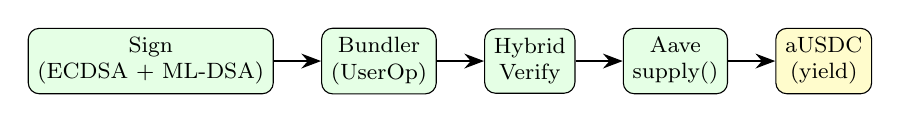
\begin{tikzpicture}[
  box/.style={draw, rounded corners, fill=green!10, minimum height=0.8cm, align=center, font=\footnotesize},
  arr/.style={-{Stealth[length=2.5mm]}, thick}
]
\node (s) [box] {Sign\\(ECDSA + ML-DSA)};
\node (b) [box, right=0.6cm of s] {Bundler\\(UserOp)};
\node (v) [box, right=0.6cm of b] {Hybrid\\Verify};
\node (a) [box, right=0.6cm of v] {Aave\\supply()};
\node (y) [box, right=0.6cm of a, fill=yellow!20] {aUSDC\\(yield)};
\draw[arr] (s)--(b); \draw[arr] (b)--(v); \draw[arr] (v)--(a); \draw[arr] (a)--(y);
\end{tikzpicture}
\end{center}

\end{frame}

\end{document}
